\documentclass[a4paper,12pt]{report}

\usepackage{alltt, fancyvrb, url}
\usepackage{graphicx}
\usepackage[utf8]{inputenc}
\usepackage{float}
\usepackage{hyperref}

% Questo commentalo se vuoi scrivere in inglese.
\usepackage[italian]{babel}

\usepackage[italian]{cleveref}

\title{Relario: Tales of Relano\\Progetto per il corso di\\``Programmazione ad Oggetti''}

\author{Lorenzo Cinelli, Mihai Mazuru, Kimi Osti, Sara Panfini}
\date{\today}


\begin{document}

\maketitle

\tableofcontents

\chapter{Analisi}


\section{Descrizione e requisiti}

Il software realizzato è un videogioco 2D con vista dall’alto. Il suo svolgimento gira attorno a un personaggio principale, controllato dall’utente, che deve attraversare le stanze di un castello per raggiungere lo scontro finale con il Re, di cui deve conquistare il trono.
%
\newline Durante l’esplorazione delle stanze all’utente potranno essere affidate delle quest da completare per poter procedere correttamente.
%
\newline Inoltre, gli verranno presentato delle stanze quasi completamente interattive. In particolare, ci saranno dei personaggi non giocanti (neutri, alleati o nemici) che potranno, al momento dell’interazione, mostrare un messaggio, donare degli oggetti oppure ingaggiare un combattimento. Inoltre, sarà possibile interagire con gran parte degli elementi di arredo presenti in stanza, tra cui elementi come armature o vasi contenenti oggetti collezionabili oppure tappeti o botole che possono celare al loro interno nemici.
%
\newline Il combattimento si svolge per turni. Ad ogni turno, il giocatore può decidere se attaccare o chiedere pietà al nemico, così come può navigare il suo inventario e usare oggetti senza perdere il diritto al turno. Il nemico, in caso venga chiesta pietà, potrebbe concederla oppure rifiutarla e attaccare immediatamente il giocatore. 

\subsubsection{Requisiti funzionali}
\begin{itemize}
	\item I nemici all'interno del gioco saranno di varie tipologie, e dovranno offrire un comportamento variabile all'utente per quanto riguarda le richieste di pietà;
	\item L'arredo delle stanze viene generato casualmente garantendo l'assenza di sovrapposizioni, e le diverse tipologie di elementi di arredo devono offrire diversi scenari di interazione;
	\item Le quest devono essere di diverse tipologie e richiedere diverse azioni da parte del giocatore;
	\item Il combattimento finale deve poter offrire una scelta al giocatore, che sarà in grado di avviare finali diversi.
\end{itemize}

\subsubsection{Requisiti non funzionali}
\begin{itemize}
	\item Per offire un'esperienza gradevole all'utente, si mira a realizzare un software efficiente.
	\item Il software sarà portabile su tutti i maggiori sistemi operativi.
\end{itemize}


\section{Modello del Dominio}

Il dominio applicativo dell’applicazione viene modellato in ogni momento dal concetto di stanza, ovvero il “container” all’interno di cui si svolge la fase centrale del gioco. All’interno della stanza, oltre al personaggio principale, si trovano altre entità, che possono essere personaggi viventi non giocanti (nemici o generici NPC) oppure elementi di arredo. Il giocatore può possedere nel suo inventario diversi oggetti, che vengono anch’essi modellati come entità. In questo scenario, diventa possibile gestire tramite la stanza e le informazioni che ogni entità offre l’intero modello del dominio, estraendo le istanze di interesse per gestire le situazioni contingenti come il combattimento. 
%
\newline Per quanto riguarda l’arredamento, le entità si dividono in tre tipologie fondamentali: arredamento interattivo, che blocca il movimento ma permette interazione, e può rilasciare un oggetto che il giocatore aggiungerà al proprio inventario al momento dell’interazione; arredamento calpestabile, che non ostruisce il movimento e permette interazione, ma può nascondere un nemico con cui viene avviato il combattimento non appena vi si interagisce; arredamento passivo, che ostacola il movimento e non permette alcun tipo di interazione. 
%
\newline Per quanto riguarda i nemici, ad ognuno viene associato un tipo, che ne definisce il livello di difficoltà. Quando viene sconfitto, un nemico rilascia un oggetto di inventario che il giocatore aggiungerà al proprio inventario al momento della vittoria. Ad ogni nemico viene poi associato un comportamento in caso di richieste di pietà, indipendente dal tipo e proprio di ogni singola istanza. In caso il giocatore venga risparmiato dal nemico, non ottiene il suo bottino.
%
\newline Gli NPC modellano tutti i personaggi non ostili all’interno del gioco, con cui sarà possibile interagire in ogni momento. Anche loro possono rilasciare oggetti di inventario al momento dell’interazione, oppure mostrare messaggi, che potranno o meno aiutare il giocatore a completare la quest.
%
\newline Il personaggio principale, che si muove nella mappa e interagisce con il resto delle entità presenti, può portare con sé alcuni oggetti di inventario ottenuti interagendo con le altre entità. Questi oggetti possono essere di vario tipo, e a seconda della tipologia offrire diversi effetti (cura, aumento del danno per le armi e protezione per le armature, oppure nessuno per gli oggetti collezionabili). Le armi e le armature, per essere effettive, devono essere equipaggiate, e hanno una durabilità limitata. Al momento dell’uso dell’oggetto, il suo effetto viene attivato sul giocatore. Un oggetto qualsiasi può anche essere scartato per liberare spazio nell’inventario, che ha capacità limitata.


\begin{figure}[H]
	\centering{}
	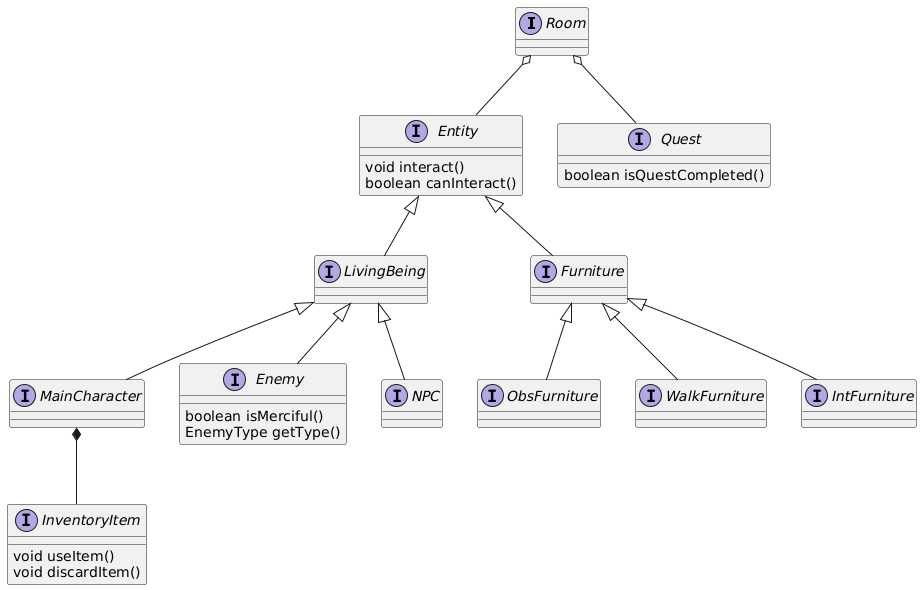
\includegraphics[width=\textwidth]{img/model.png}
	\caption{Schema UML del dominio applicativo}
	\label{img:model}
\end{figure}


\chapter{Design}

\section{Architettura}

Il software si basa sull’architettura MVC nella sua declinazione standard. In particolare, ogni elemento dell’architettura offre un unico entry point verso l’esterno, in modo che gli accessi alle sue funzionalità possano essere uniformi e consistenti, offrendo un ulteriore grado di incapsulamento.
%
\newline Il Model offre come proprio entry point l’interfaccia Room, che fa da scenario base per lo svolgimento della fase di esplorazione del gioco. All’interno della stanza infatti, sono presenti tutte le entità, che vengono modificate ad ogni tick del motore fisico tramite un metodo offerto dalla stessa Room, deputata a controllare anche se le singole entità siano in grado di muoversi al suo interno. 
%
\newline Il Controller, che conserva il riferimento alla stanza in cui attualmente si trova il gioco, gestisce al suo interno le transizioni di stato per le varie fasi del gameplay, interrogando la View per mostrare le interfacce corrette e richiedendo al Model eventuali modifiche. Il Controller è anche responsabile della temporizzazione dell’aggiornamento del motore di gioco, e della traduzione delle entità del Model in elementi rappresentabili correttamente dalla View.
%
\newline La View offre un entry point centrale da cui è possibile richiedere di mostrare le varie interfacce, o l’accesso ai loro riferimenti per chiamare procedure proprie di tali istanze. Nell’architettura realizzata, la View agisce come elemento passivo ricevendo i dati da mostrare dal Controller tramite opportune interrogazioni. La gestione dell’input permette alla View di comunicare particolari eventi al Controller, che li gestirà e ne rifletterà eventualmente gli effetti sul Model.
%
\newline Nella realizzazione dell’architettura MVC, modificare la View non impatta minimamente il Model, dal momento che è solamente il Controller a dialogare con questa componente. Dall’altro lato, il Controller potrebbe essere impattato da una modifica della View radicale (come per esempio trasformare la GUI attiva in un’interfaccia reattiva, oppure la rimozione dei suoni), mentre non sarebbe impattato da modifiche nelle tecniche implementative della GUI - come per esempio una modifica della libreria grafica - a patto che sia in grado di rispettare il contratto stabilito dalle due interfacce (ad esempio accettare gli stessi tipi di chiamate parametrizzate).


\begin{figure}[H]
	\centering{}
	
	\caption{Schema UML degli entry point dei rapporti fra componenti di MVC}
	\label{img:mvc}
\end{figure}

\section{Design dettagliato}

\subsection{Sara Panfini}
\subsection{\textbf{Gestione dei Nemici}}
\textbf{Problema:} Il problema da affrontare è la gestione dei nemici, che possono avere caratteristiche variabili, come
la vita, il danno o gli oggetti che offrono come ricompensa dopo un combattimento, in base alla loro tipologia e livello di difficoltà.
Inoltre, la creazione dei nemici dovrebbe essere gestita in modo da poter essere facilmente estendibile, così da consentire l'aggiunta
di nuove tipologie di nemici senza dover necessariamente modificare il codice già esistente.\newline
\textbf{Soluzione:} La soluzione adottata è quella di utilizzare il \textit{Factory Pattern} e implementare una factory di nemici nell'interfaccia
\textit{EnemyFactory} e nella sua relativa implementazione \textit{EnemyFactoryImpl}. Inoltre, sono state sfruttate delle enumerazioni per
gestire le varie tipologie e difficoltà dei nemici. Questa soluzione è stata scelta per rendere la creazione più flessibile e modulare, centralizzando
la logica di creazione dei nemici in modo da avere un sistema maggiormente scalabile.\newline

\begin{figure}[H]
	\centering{}
	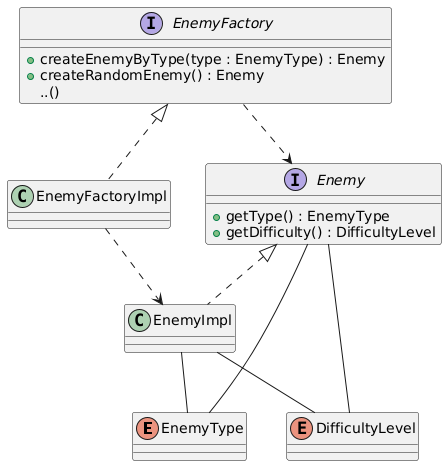
\includegraphics[width=\textwidth]{img/EnemyUML.png}
	\caption{Schema UML della Factory dei nemici}
\end{figure}


\subsection{\textbf{Gestione degli NPC neutri}}
\textbf{Problema:} Durante il gioco gli NPC sono in grado di supportare diversi tipi di interazione; ad esempio, possono regalare oggetti o assegnare le quest al giocatore.
Il sistema dovrebbe, quindi, gestire i diversi comportamenti in maniera efficiente, cioè in modo che sia possibile facilmente nuove tipologie di interazioni.\newline
\textbf{Soluzione:} Per riuscire a gestire al meglio i comportamenti variabili degli NPC, è stato utilizzato lo \textit{Strategy Pattern}.
In questo modo si riescono a stabilire diverse tipologie di comportamenti che questi personaggi possono assumere in risposta all'interazione con il giocatore.
In particolare, l'interfaccia \textit{NpcBehavior} offre un metodo base per interagire con tutti gli NPC e deve essere poi implementata dalle classi che vanno a gestire 
le specifiche tipologie di comportamento (\textit{DefaultBehavior}, \textit{LootBehavior}, ...). 
Inoltre, per crearli (con i comportamenti predefiniti) viene nuovamente utilizzato il \textit{Factory Pattern}. 
Questa soluzione implementativa rende la gestione degli NPC facilmente estendibile, dato che per definire ulteriori comportamenti si possono direttamente 
creare nuove particolari implementazioni dell'interfaccia \textit{NpcBehavior} e l'intera logica di creazione degli NPC si trova nella classe \textit{NpcFactoryImpl}.\newline

\begin{figure}[H]
	\centering{}
	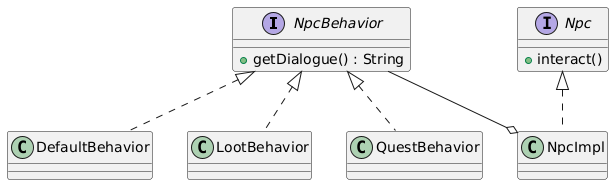
\includegraphics[width=\textwidth]{img/NpcUML.png}
	\caption{Schema UML della Factory dei nemici}
\end{figure}

\subsection{\textbf{Gestione della mappa di gioco}}
\textbf{Problema:} La problematica da affrontare è la gestione delle stanze del castello (mappa del gioco).
Durante la sua avventura, il giocatore deve, infatti, essere in grado di esplorare le diverse stanze, ognuna delle quali 
ha al suo interno elementi di arredo e personaggi non giocanti con cui è possibile interagire.
Il sistema deve, perciò, essere in grado di garantire un corretto posizionamento e anche una distribuzione logica di tutte le entità entro i confini della stanza.
In aggiunta, è necessario avere un sistema che gestisca l'eventuale assegnazione delle quest a ciascun ambiente di gioco.\newline
\textbf{Soluzione:} La soluzione proposta prevede l'implementazione dell'interfaccia \textit{Room} e della relativa classe.
Questa classe fornisce la rappresentazione di una generica stanza e si occupa di mantenere tutte le entità presenti e la loro relativa posizione al suo interno, sfruttando anche
l'enumerazione \textit{CellType} che gestisce lo stato di ogni cella della mappa.
La creazione delle stanze viene realizzata dalla classe \textit{RoomGenerator}, che ne gestisce anche il popolamento e l'eventuale assegnazione delle quest.
Per gestire le quest è stata realizzata la classe \textit{QuestManager}, che si occupa di associare o meno una specifica missione ad ogni stanza.
Questa soluzione permette di racchiudere in una unica classe l'intera logica di assegnazione delle quest e ne facilita anche l'introduzione di nuove tipologie.
Per popolare ciascuna stanza vengono usate le classi \textit{FurnitureGenerator} e \textit{LivingBeingsGenerator}.
Queste classi si occupano della generazione e della disposizione, in maniera pseudo-casuale, di tutte le entità - attraverso l'uso delle specifiche \textit{Factory} -, verificando la validità e la disponibilità
delle posizioni che gli vengono assegnate. La classe \textit{LivingBeingsGenerator}, inoltre, sfrutta una logica di suddivisione di ciascuna stanza in aree per fare in modo che la 
distribuzione dei personaggi sia in linea di massima equilibrata.
Con questo approccio si è cercato di ottenere una generazione delle stanze abbastanza dinamica, che consente, cioè, di averne configurazioni diverse, 
e di centralizzare la logica necessaria in modo da agevolare anche future possibili modifiche.\newline

\begin{figure}[H]
	\centering{}
	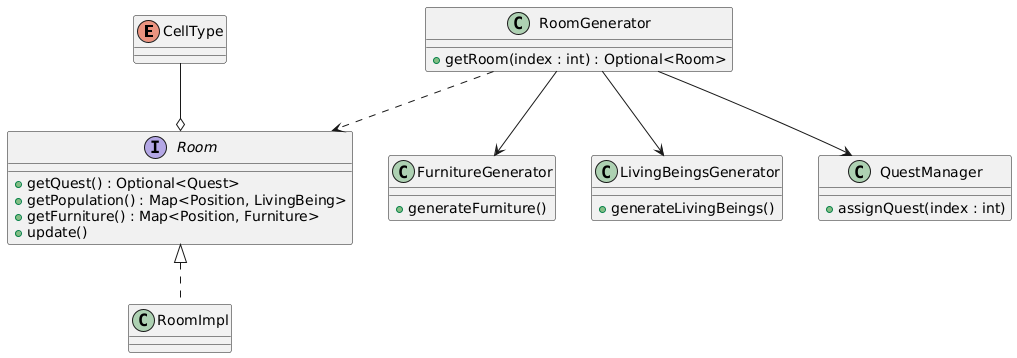
\includegraphics[width=\textwidth]{img/RoomUML.png}
	\caption{Schema UML della Factory dei nemici}
\end{figure}

\subsection{\textbf{Gestione delle Quest}}
\textbf{Problema:} Il problema è gestire le varie tipologie di quest assegnate alle stanze del gioco. È necessario creare un sistema che consenta di definire 
e verificare il completamento di ogni tipo di quest cercando di evitare ripetizioni di codice e di avere una buona estendibilità.\newline
\textbf{Soluzione:} Come per gli NPC, anche in questo caso si è fatto uso dello \textit{Strategy Pattern} per modellare il concetto di obiettivo.
Si ha, quindi, l'interfaccia \textit{ObjectiveStrategy} che viene implementata dalle classi che rappresentano gli specifici obiettivi da completare per superare le quest.
In questo modo, la singola classe \textit{QuestImpl} riesce a gestire tutte le tipologie di quest.\newline

\chapter{Sviluppo}
\section{Testing automatizzato}

Per quanto riguarda il testing automatizzato, si è sfruttata la libreria JUnit e si sono realizzati test su quasi tutte le classi di Model e Controller. Ciò è stato fatto per garantire il corretto funzionamento dell’applicazione, e per avere la certezza che gli eventuali problemi riscontrati durante il gioco non fossero dovuti a mancanze di logica implementativa, quanto a problematiche di visualizzazione. 
%
\newline La View, invece, è stata testata manualmente in fase di sviluppo, e poi in fase di collaudo del software, perché personalmente non siamo riusciti ad approfondire le dinamiche di testing automatizzato che avrebbero permesso di testare automaticamente anche quella parte del software.
%
\newline In linea generale, gli aspetti su cui il testing si è maggiormente soffermato sono stati i seguenti:

\begin{itemize}
	\item Generazione della mappa, movimento e interazioni al suo interno. Particolarmente, si è verificato che il movimento e le interazioni non generassero comportamenti imprevisti e che si riflettessero correttamente sugli aggiornamenti del Model.
	\item Combattimento. In particolare, il testing si concentra sul mantenimento dell’ordine dei turni per evitare comportamenti imprevisti, e sul corretto inserimento in inventario del bottino dei nemici sconfitti.
	\item Protagonista. In particolare, si è testato il sistema di gestione della vita del protagonista, così come del suo inventario. Nei controlli sull’inventario, si è verificato il corretto utilizzo degli oggetti curativi, così come delle armi e armature, per garantire comportamenti consistenti in fase di combattimento.
	\item Input utente. Si sono testati i Controller che svolgono la funzione di Observer, per garantire la corretta gestione degli input.
	\item Creazione delle istanze. Avendo fatto largo uso del Pattern Factory, si è deciso di testare i metodi di generazione degli oggetti per verificare l’effettiva consistenza delle istanze create e garantire prevedibilità in fase di gioco.
\end{itemize}

\section{Note di sviluppo}

\subsection{\textbf{Sara Panfini}}
Seguono alcuni esempi di parti di codice con funzionalità avanzate.
\begin{itemize}
	\item \textbf{Espressioni Lambda e Stream}
	https://github.com/KimboCoffee/OOP23-relario/blob/cb9e0fd37a803cebfb509ff1b08d7df99b5ee8fc/src/main/java/it/unibo/oop/relario/model/inventory/InventoryItemFactoryImpl.java#L84-L86
	https://github.com/KimboCoffee/OOP23-relario/blob/cb9e0fd37a803cebfb509ff1b08d7df99b5ee8fc/src/main/java/it/unibo/oop/relario/model/map/RoomImpl.java#L158-L161
	https://github.com/KimboCoffee/OOP23-relario/blob/cb9e0fd37a803cebfb509ff1b08d7df99b5ee8fc/src/main/java/it/unibo/oop/relario/model/quest/DefeatEnemyObjective.java#L32-L35
	\item \textbf{Optional}
	https://github.com/KimboCoffee/OOP23-relario/blob/cb9e0fd37a803cebfb509ff1b08d7df99b5ee8fc/src/main/java/it/unibo/oop/relario/model/map/QuestManager.java#L73-L74
	https://github.com/KimboCoffee/OOP23-relario/blob/cb9e0fd37a803cebfb509ff1b08d7df99b5ee8fc/src/main/java/it/unibo/oop/relario/model/map/RoomGenerator.java#L57-L58
	https://github.com/KimboCoffee/OOP23-relario/blob/cb9e0fd37a803cebfb509ff1b08d7df99b5ee8fc/src/main/java/it/unibo/oop/relario/model/map/FurnitureGenerator.java#L55
	\item \textbf{Record}
	https://github.com/KimboCoffee/OOP23-relario/blob/cb9e0fd37a803cebfb509ff1b08d7df99b5ee8fc/src/main/java/it/unibo/oop/relario/model/entities/enemies/EnemyFactoryImpl.java#L100
	\item \textbf{Java Wildcards}
	https://github.com/KimboCoffee/OOP23-relario/blob/cb9e0fd37a803cebfb509ff1b08d7df99b5ee8fc/src/main/java/it/unibo/oop/relario/model/quest/ObjectiveStrategy.java#L25
\end{itemize}
\newline
\textbf{Codice preso da altri}
Per la realizzazione della classe \textit{Pair}: https://bitbucket.org/mviroli/oop2023-esami/src/c5edbdde70b6a4ead339098297c82ca7372c96f6/a01a/e1/Pair.java#lines-9:55


\chapter{Commenti finali}
\subsection{Autovalutazione e lavori futuri}

\subsection{Sara Panfini}
Questo progetto è stato sicuramente uno degli scogli più grandi che ho dovuto affrontare nel 
mio percorso fino ad ora. Inizialmente, non mi sentivo preparata e non credevo di avere le conoscenze
per affrontare un progetto di questa portata. Ciò ha reso le prime fasi di lavoro particolarmente complesse
per me e, perciò, durante quel periodo sento di non aver contribuito abbastanza e di non 
essere stata di grande aiuto al gruppo. Con il tempo, però, sono riuscita a prendere consapevolezza e ritengo
di essere stata in grado di apportare un buon contributo al progetto, anche se avrei sicuramente potuto gestire 
meglio alcune cose, come l'organizzazione del lavoro e la gestione dei tempi.\newline
Nonostante, generalmente, io non mi trovi a mio agio con i lavori di gruppo, considero questa comunque come
un'esperienza, nel complesso, positiva. Ci sono, ovviamente, state opinioni contrastanti su alcuni aspetti
dello sviluppo del progetto, ma, nonostante ciò, abbiamo sempre cercato di lavorare insieme nel rispetto degli 
altri componenti del gruppo.\newline
In generale, quindi, questo progetto ha rappresentato una grande sfida per me e, a prescindere dalle varie
difficoltà, sono soddisfatta di come sono riuscita ad affrontarla. Lavorare allo sviluppo di un sistema di queste
dimensioni mi ha stimolato molto e mi ha anche iniziato al mondo dei videogiochi, che non conoscevo e che ora mi affascina molto.
Nel complesso, credo che questa esperienza mi abbia fatto imparare molto e mi abbia fornito gli strumenti 
per riuscire ad affrontare progetti futuri con maggiore preparazione e con un approccio più consapevole.\newline

\appendix
\chapter{Guida utente}

Capitolo in cui si spiega come utilizzare il software. Nel caso in cui il suo uso sia del tutto
banale, tale capitolo può essere omesso.
%
A tal riguardo, si fa presente agli studenti che i docenti non hanno mai utilizzato il software
prima, per cui aspetti che sembrano del tutto banali a chi ha sviluppato l'applicazione possono non
esserlo per chi la usa per la prima volta.
%
Se, ad esempio, per cominciare una partita con un videogioco è necessario premere la barra
spaziatrice, o il tasto ``P'', è necessario che gli studenti lo segnalino.

\subsection*{Elementi positivi}

\begin{itemize}
 \item Si istruisce in modo semplice l'utente sull'uso dell'applicazione, eventualmente facendo uso di schermate e descrizioni.
\end{itemize}

\subsection*{Elementi negativi}
\begin{itemize}
 \item Si descrivono in modo eccessivamente minuzioso tutte le caratteristiche, anche minori, del software in oggetto.
 \item Manca una descrizione che consenta ad un utente qualunque di utilizzare almeno le funzionalità primarie dell'applicativo.
\end{itemize}

\chapter{Esercitazioni di laboratorio}

In questo capitolo ciascuno studente elenca gli esercizi di laboratorio che ha svolto
(se ne ha svolti),
elencando i permalink dei post sul forum dove è avvenuta la consegna.
%
Questa sezione potrebbe essere processata da strumenti automatici,
per cui link a oggetti diversi dal permalink della consegna,
errori nell'email o nel nome del laboratorio possono portare ad ignorare alcune consegne,
si raccomanda la massima precisione.

\section*{Esempio}

\subsection{paolino.paperino@studio.unibo.it}

\begin{itemize}
 \item Laboratorio 04: \url{https://virtuale.unibo.it/mod/forum/discuss.php?d=12345#p123456}
 \item Laboratorio 06: \url{https://virtuale.unibo.it/mod/forum/discuss.php?d=22222#p222222}
 \item Laboratorio 09: \url{https://virtuale.unibo.it/mod/forum/discuss.php?d=99999#p999999}
\end{itemize}

\subsection{paperon.depaperoni@studio.unibo.it}

\begin{itemize}
 \item Laboratorio 04: \url{https://virtuale.unibo.it/mod/forum/discuss.php?d=12345#p123456}
 \item Laboratorio 05: \url{https://virtuale.unibo.it/mod/forum/discuss.php?d=22222#p222222}
 \item Laboratorio 06: \url{https://virtuale.unibo.it/mod/forum/discuss.php?d=99999#p999999}
 \item Laboratorio 07: \url{https://virtuale.unibo.it/mod/forum/discuss.php?d=22222#p222222}
 \item Laboratorio 08: \url{https://virtuale.unibo.it/mod/forum/discuss.php?d=99999#p999999}
 \item Laboratorio 09: \url{https://virtuale.unibo.it/mod/forum/discuss.php?d=22222#p222222}
 \item Laboratorio 10: \url{https://virtuale.unibo.it/mod/forum/discuss.php?d=99999#p999999}
 \item Laboratorio 11: \url{https://virtuale.unibo.it/mod/forum/discuss.php?d=22222#p222222}
\end{itemize}


\bibliographystyle{alpha}
\bibliography{13-template}

\end{document}
